	\documentclass[10pt,oneside]{CBFT_book}
	% Algunos paquetes
	\usepackage{amssymb}
	\usepackage{amsmath}
	\usepackage{graphicx}
% 	\usepackage{libertine}
% 	\usepackage[bold-style=TeX]{unicode-math}
	\usepackage{lipsum}

	\usepackage{natbib}
	\setcitestyle{square}

	\usepackage{polyglossia}
	\setdefaultlanguage{spanish}
	



	\usepackage{CBFT.estilo} % Cargo la hoja de estilo

	% Tipografías
	% \setromanfont[Mapping=tex-text]{Linux Libertine O}
	% \setsansfont[Mapping=tex-text]{DejaVu Sans}
	% \setmonofont[Mapping=tex-text]{DejaVu Sans Mono}

	%===================================================================
	%	DOCUMENTO PROPIAMENTE DICHO
	%===================================================================

\begin{document}

% =================================================================================================
\chapter{Teorema de Wigner-Eckart}
% =================================================================================================

Este teorema facilita el cálculo de elementos de matriz de un tensor.
Un operador cualquiera puede descomponerse tensorialmente.
Es importante para el cálculo de transiciones evaluar elementos de matriz de operadores tensoriales.
Si determino qué coeficientes son nulos entonces eso significa que no hay probabilidad entre ellos.

Los elementos matriciales de operadores tensoriales respecto de autoestados de momento satisfacen 
\[
	\Braket{\alpha',j',m'|T^{(k)}_q|\alpha,j,m} =  \Braket{j k; m q | j k; j' m'}
	\frac{\Braket{\alpha' j'|T^{(k)}|\alpha j}}{(2j+1)}
\]
un coeficiente que no depende de $q,m,m'$. El coeficiente que aparece primero es el coeficiente de 
Clebsh-Goran de sumar momentos $jk$ con $m_1=m, m_2=q, m+q=m'$ .

La regla de selección se construye 
\[
	\Braket{\alpha',j',m'|[J_z, T^{(k)}_q] - \hbar q T^{(k)}_q |\alpha,j,m} = 
	\Braket{|J_z T^{(k)}_q - T^{(k)}_q J_z - \hbar q T^{(k)}_q|} = 0
\]
\[
	\Braket{\alpha',j',m'|0|\alpha,j,m} = 
	(\hbar m' - \hbar m -\hbar q )\Braket{\alpha',j',m'|T^{(k)}_q|\alpha,j,m}
\]
\[
	0 = \hbar ( m' - m - q ) \Braket{\alpha',j',m'|T^{(k)}_q|\alpha,j,m}
\]
\[
	\text{si} \; m' \neq m+q \longrightarrow \Braket{\alpha',j',m'|T^{(k)}_q|\alpha,j,m} = 0
\]
Este coeficientes será nulo si $m' = m+q$ pués $T_q^{(k)}\Ket{\a,j,m} \propto \Ket{\a,j,m+q}$

El teorema nos dice que
\be
	\Braket{\alpha',j',m'|T^{(k)}_q|\alpha,j,m} =  \Braket{j, k; m, q | j, k; j', m'}
	\frac{\Braket{\alpha', j'|T^{(k)}|\alpha, j}}{(2j+1)}
	\label{resultado_teorema_wigner}
\ee
donde el valor de este último coeficiente es independiente de la componente $q$ y de $m, m'$.
Estos elementos de matriz tienen reglas de selección parecidas a las de los coeficientes de
Clebsh-Gordan.
En efecto, la expresión \eqref{resultado_teorema_wigner} será nula salvo cuando $m'= m+q, 
|j-k| \leq j' \leq j + k$. Veamos cómo demostrar dicha expresión.

Una idea de la demostración del teorema parte de que 
\begin{multline*}
	\Braket{\alpha',j',m'|[J_\pm ,T^{(k)}_q]|\alpha,j,m} = \\
	\hbar\sqrt{(k\mp q)(k\pm q + 1)} 
	\Braket{\alpha',j',m'|T^{(k)}_{q\pm 1}|\alpha,j,m} 
\end{multline*}
que se descompone a 
\begin{multline*}
	\sqrt{(j'\pm m')(j'\mp m' + 1)} \Braket{\alpha',j',m'\pm 1|T^{(k)}_q|\alpha,j,m} - \\
	\sqrt{(j'\mp m')(j'\pm m' + 1)} \Braket{\alpha',j',m'|T^{(k)}_q|\alpha,j,m \pm 1} = \\
	\sqrt{(k\mp q)(k\pm q + 1)}  \Braket{\alpha',j',m'|T^{(k)}_{q\pm 1}|\alpha,j,m}.
\end{multline*}

Pero ésta es la misma relación de recurrencia vista para los coeficientes de Clebsh-Gordan, 
si reemplazamos
\[
	m'=m \quad j=j_1 \quad m=m_1 \qquad j'=j \quad k=j_2 \quad q=m_2
\]

Como ambas relaciones son lineales, sus resultados serán proporcionales. Se puede asociar 
\[
	\Braket{ j_1, j_2 ; m_1, m_2 \pm 1 | j_1, j_2 ; j, m} \propto 
	\Braket{\alpha',j',m'|T^{(k)}_{q\pm 1}|\alpha,j,m}
\]
\[
	\Braket{ j_1, k ; m, q \pm 1 | j, k ; j', m'} \propto 
	\Braket{\alpha',j',m'|T^{(k)}_{q\pm 1}|\alpha,j,m}
\]
Logramos la igualdad metiendo una constante $C(j,j',k)$ independiente de $m',q,m$ de tal manera
que
\begin{multline*}
	\Braket{\alpha',j',m'|T^{(k)}_{q\pm 1}|\alpha,j,m}
	\Braket{ j_1, j_2 ; m_1, m_2 \pm 1 | j_1, j_2 ; j, m} = \\
	\Braket{ j_1, k ; m, q \pm 1 | j, k ; j', m'} \: C(j,j',k).
\end{multline*}

Asimismo, como se tiene a $\Braket{|T_q^{(k)}|}$ proporcional a los coeficientes de Clebsh-Gordan, 
serán válidas las mismas reglas de selección 
\[
	m' = m + q \qquad |j-k| \leq j' \leq j+k.
\]

\begin{ejemplo}{\bf Ejemplo del teorema para escalares y vectores}

Sea un escalar (número), o bien un tensor de rango cero $S=T_0^{(0)}$, entonces
\[
	\Braket{\alpha', j', m' |T_0^{(0)}| \alpha, j, m} \propto 
	\Braket{j, 0 ; m, 0 |j, 0 ; j', m'} = \delta_{j'j}\delta_{m'm} 
\]
que es el coeficiente de Clebsh-Gordan de sumar $j+0=j$, salvo que $j=j'$ es nulo,
por lo cual aparece $\delta_{j'j}$; pero $m+0 = m = m'$ y entonces
\[
	\Braket{\alpha', j', m' |T_0^{(0)}| \alpha, j, m} =
	\delta_{j'j}\delta_{m'm}  \frac{\Braket{\a',j'|S|\a,j}}{\sqrt{2j+1}}
\]
se ve que el $S$ no conecta estados con $m,j$ diferentes. La transición es independiente de
$m$ lo cual puede mostrarse así
% \[
% 	q=0 \; k=0 \quad m+q=m' \rightarrow m=m'
% \]
% \[
% 	|j-0| \leq j' \leq j+0 \rightarrow j=j'
% \]
% No varían $j,m$ en los estados No conecta estados con $j,m$ diferentes un escalar.
\[
	(j=5,m=5) \to (j=5,m=5) \equiv (j=5,m=4) \to (j=5,m=4).
\]

Sea ahora un vector (tensor de rango uno):
\[
	\Braket{\alpha', j', m'|T_q^{(1)}| \alpha, j, m} 
	\propto \Braket{j, 1 ; m , q | j, 1 ; j', m'}
\]
Como $k=1$ se tienen $q=1,0,-1$, lo cual conduce a que
\[
	|j-1| \leq j' \leq j+1 \quad -1\leq j'-j \leq 1 
	\qquad \rightarrow  \qquad 
	j-j'=\begin{cases} 1 \\ 0 \\ -1 \end{cases}
\]
\[
	m + \{1,0,-1\} = m' \qquad \rightarrow \qquad 
	m - m' =\begin{cases} 1 \\ 0 \\ -1 \end{cases}
\]

Entonces, el vector conectará estados con $j-j' = \pm 1, 0$. No produce transiciones entre
$j$ y $j'$ alejados en más de una unidad. Para $m$ tendré lo mismo.
La constante que completa la proporcionalidad será la misma para varios coeficientes.
Esto tiene suma importancia en la conexión de estados $j=0+1=1$.

\end{ejemplo}

\section{Teorema de proyección}

Consideremos lo que sucede en el teorema de Wigner-Eckart si $j=j'$ y se lo aplicamos a un operador vectorial 
$T_q^{(k=1)} \equiv V_q$
\[
	\Braket{\alpha', j, m'|V_q|\alpha, j, m} = 
	\frac{\Braket{\alpha', j, m|\vb{J}\cdot\vb{V}|\alpha, j, m}}{\hbar^2j(j+1)}\Braket{j, m'|J_q|j, m}.
\]

Como caso especial, si $\alpha' =\alpha$ estoy en un subespacio donde coinciden los números cuánticos
salvo $m$. Allí vale que 
\[
	\vb{V}_{\a,j} = \frac{ \Braket{\vb{J}\cdot\vb{V}}_{\a,j} }{\hbar^2j(j+1)} \vb{J},
\]
donde los subíndices $\a,j$ implican respecto a quien estoy tomando valor medio. Esto vale para cualquier
vector en el mismo subespacio,
\[
	\vb{V} = \frac{\Braket{\vb{J}\cdot\vb{V}}}{\hbar^2j(j+1)} \vb{J}.
\]

Intentemos probar esto. Reescribimos, con otra normalización, lo siguiente:
\[
	\pe{J}{V} = J_0 V_0 - J_{+1} V_{-1} - J_{-1} V_{+1}
\]
\[
	V_{\pm 1} = \mp \frac{1}{\sqrt{2}}( V_x \pm i V_y)
\]
\[
	V_0 = V_z, \; J_{\pm 1} = \mp \frac{1}{\sqrt{2}} J_{\pm}, J_0 = J_z
\]
y luego
\begin{multline*}
 \Braket{ \a', j, m | \pe{J}{V} | \a, j, m } = m \hbar \Braket{ \a', j, m | V_0 | \a, j, m } + \\
	\frac{\hbar}{\sqrt{2}} \sqrt{(j-m)(j-m+1)} \Braket{ \a', j, m-1 | V_{-1} | \a, j, m } + \\
	- \frac{\hbar}{\sqrt{2}} \sqrt{(j-m)(j+m+1)} \Braket{ \a', j, m+1 | V_{+1} | \a, j, m }
\end{multline*}

Cada una de las tres componentes del segundo miembreo es proporcional a $\Braket{}$ lo que lleva a
\[
	\Braket{ \a', j, m | \pe{J}{V} | \a', j, m } = C_{j,m} \Braket{ \a, j || \vb V || \a, j }
\]
donde $C_{jm}$ ren realidad solo depende de $j$. Consideremos ahora $\vb V = \vb J$ y $\a = \a'$
(nos metemos en un subespacio).
\[
	\Braket{ \a, j, m | \vb J^2 | \a, j, m } = C_j \Braket{ \a, j || \vb V || \a, j }
\]
y entonces
\[
	\frac{\Braket{ \a', j, m' | \pe{J}{V} | \a, j, m }}{\Braket{ \a, j, m' | \vb J^2 | \a, j, m }} = 
	\frac{\Braket{ \a', j || \vb V || \a, j }}{\Braket{ \a, j || \vb J || \a, j }}.
\]
Ahora introducimos el teorema de Wigner-Eckart,
\[
	\frac{\Braket{ \a', j, m' | V_q | \a, j, m }}{\Braket{ \a, j, m' | J_q | \a, j, m }} = 
	\frac{\Braket{ \a', j || \vb V || \a, j }}{\Braket{ \a, j || \vb J || \a, j }}
	\frac{ \text{CG } (2j+1)^{-1/2}}{\text{CG } (2j+1)^{-1/2} }
\]
\[
	\Braket{ \a', j, m' | V_q | \a, j, m } =
	\frac{\Braket{ \a', j, m' | \pe{J}{V} | \a, j, m }}{\hbar^2 \: j (j+1)}
	\Braket{ \a, j, m' | J_q | \a, j, m }
\]
Puede pensarlo como $\Ket{\a,j,m} = \Ket{\a,j}\otimes\Ket{m}$ y 
\[
	\Braket{ \a, j |\Braket{j,m'|V_q|\a,j} | j,m } \propto \Braket{\a,j|\pe{J}{V}|\a,j},
\]
siendo el yeite el hecho de que dentro de un subepsacio todos los vectores son proporcionales
entre sí.


\subsection{Aplicación del teorema de proyección}

Sea un $H_0$ coulombiano esféricamente simétrico $[H_0,\vb{J}]=0$ , $\vb{J}=\vb{L}+\vb{S}$ y $J^2=(L+S)^2$
\[
	H_0 = \frac{p^2}{2m} + \frac{e}{r} \qquad \Ket{E,\ell,s,j,m} \quad 2j+1 \;\text{degenerados}
\]
que equivale a un $CCOC:H,L^2,S^2,J^2,J_z$ donde cada autovalor dentro del ket es el que corresponde a estos 
operadores.

Si meto un campo $B$ en $\hat{z}$ tendré 
\[
	H \equiv H_0 + H_1 = H_0 - \frac{\mu_B B}{\hbar}(L_z + 2S_z)
\]
\notamargen{El factor 2 que acompaña al $S_z$ no es una boludez demostrarlo; es el factor giromagnético
de Landé.}
lo cual debería romper la degeneración.
Pero este factor $2$ no puedo saber cómo operarlo porque los números cuánticos $E,\ell,s,j,m$ no dan
manera de sperarar cuanto de $L_z$ y cuańto de $S_z$, pues asocié $j$ a $\vb J = \vb L + \vb S$ y no a 
$\vb J = \vb L + 2 \vb S$\footnote{Podría hacerlo con {\it brute force} pasando a una base desacoplada
donde tengo $m_{\ell}$ y $m_s$ como números cuánticos.}.

Utilizando el teorema de proyección para escribir $\vb L$  y $\vb S$ en términos de $\vb J$ se puede
escribir
\[
	L_z + 2S_z = \frac{\Braket{\vb{J}\cdot\vb{L}}}{\hbar^2j(j+1)}J_z + 
		2\frac{\Braket{\vb{S}\cdot\vb{J}}}{\hbar^2j(j+1)}J_z
\]
pero no puedo poner este nuevo operador, que mete el campo B, en el CCOC directamente, entonces uso teorema 
de proyección.
\[
	\vb{J}\cdot\vb{L} = L^2 + \frac{1}{2}( J^2 - L^2 - S^2 )
\]
\[
	\vb{J}\cdot\vb{S} = S^2 + \frac{1}{2}( J^2 - L^2 - S^2 )
\]
Entonces tengo todo expresado en función de $J_z$ que sí forma parte de mi CCOC.

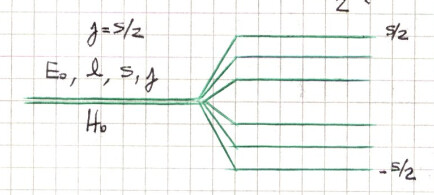
\includegraphics[width=0.5\textwidth]{images/fig_ft2_H_proy.jpg}

\begin{ejemplo}{\bf Ejercicio}
 
\end{ejemplo}

\begin{ejemplo}{\bf Ejercicio}
 
\end{ejemplo}


\begin{ejemplo}{\bf Ejercicio}
 
\end{ejemplo}



% \bibliographystyle{CBFT-apa-good}	% (uses file "apa-good.bst")
% \bibliography{CBFT.Referencias} % La base de datos bibliográfica

\end{document}
